%
%  =======================================================================
%  ····Y88b···d88P················888b·····d888·d8b·······················
%  ·····Y88b·d88P·················8888b···d8888·Y8P·······················
%  ······Y88o88P··················88888b·d88888···························
%  ·······Y888P··8888b···88888b···888Y88888P888·888·88888b·····d88b·······
%  ········888······"88b·888·"88b·888·Y888P·888·888·888·"88b·d88P"88b·····
%  ········888···d888888·888··888·888··Y8P··888·888·888··888·888··888·····
%  ········888··888··888·888··888·888···"···888·888·888··888·Y88b·888·····
%  ········888··"Y888888·888··888·888·······888·888·888··888··"Y88888·····
%  ·······························································888·····
%  ··························································Y8b·d88P·····
%  ···························································"Y88P"······
%  =======================================================================
% 
%  -----------------------------------------------------------------------
% Author       : 焱铭
% Date         : 2023-08-07 14:48:16 +0800
% LastEditTime : 2023-08-19 21:15:25 +0800
% Github       : https://github.com/YanMing-lxb/
% FilePath     : \YM-CV-Template\YM-CV.tex
% Description  : 
%  -----------------------------------------------------------------------
%

\documentclass[a4paper,11pt]{ctexart}
\usepackage{YM-CV-Style}

% ============================================= 个人信息 ============================================
\newcommand{\name}{\textbf{\textbf{焱铭}}} % Your Name
\newcommand{\politicalprofile}{政治身份} % Your Course
\newcommand{\graduateschool}{桂林电子科技大学}
\newcommand{\age}{25岁}
\newcommand{\phone}{138XXXX3919} % Your Phone Number
\newcommand{\wechat}{lxb-XXXX}
\newcommand{\email}{lxb-XXXX@foxmail.com} %Email
\newcommand{\github}{https://github.com/YanMing-lxb} %Github




\begin{document}

% ============================================= 头部信息 ============================================
\parbox{2.35cm}{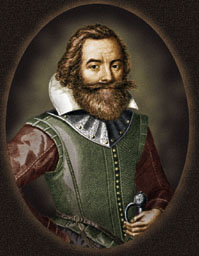
\includegraphics[width=2cm,clip]{./Picture/Photo.jpg}}
\parbox{\dimexpr\linewidth-2.8cm\relax}{
  \begin{tabularx}{\linewidth}{L r l}
    \textbf{\LARGE \name} & \faPhone\enspace    & \phone                       \\
    \age                  & \faWeixin\enspace   & \wechat                      \\
    \politicalprofile     & \faEnvelope\enspace & \href{mailto:\email}{\email} \\
    \graduateschool       & \faGithub\enspace   & \href{\github}{GitHub}
  \end{tabularx}
}
\vspace{-2mm}




% ============================================= 教育背景 ============================================
\section{\texorpdfstring{\faUniversity\,}{} 教育背景}

\setlength{\tabcolsep}{5pt}

% ---------- 有两种三种风格,请根据自己的喜好解除注释 ----------
% 风格一
\small{
\begin{tabularx}
  {\dimexpr\textwidth\relax}{lLr}
  \multirow{2}{*}{
\includegraphics[width=2.5em]{./Picture/GUET-LOGO.pdf}} & \textbf{桂林电子科技大学}          & \multirow{2}{*}{\footnotesize\textit{2020.09 - 2023.06}} \\
                                                              & 机电工程学院|机械工程专业|学术型硕士学位      &                                                          \\
  \multirow{2}{*}{
\includegraphics[width=2.5em]{./Picture/HUC-LOGO.pdf}}  & \textbf{哈尔滨商业大学}           & \multirow{2}{*}{\footnotesize\textit{2016.09 - 2020.06}} \\
                                                              & 轻工学院|机械设计制造及其自动化\&金融学|学士学位 &                                                          \\
\end{tabularx}
  }

% 风格二
% \small{
%   \begin{tabularx}
%     {\dimexpr\textwidth\relax}{Lr}
%     \textbf{桂林电子科技大学}          & \multirow{2}{*}{\footnotesize\textit{2020.09 - 2023.06}} \\
%     机电工程学院|机械工程|学术型硕士学位   &                                                          \\
%     \textbf{哈尔滨商业大学}           & \multirow{2}{*}{\footnotesize\textit{2016.09 - 2020.06}} \\
%     轻工学院|机械设计制造及其自动化\&金融学|学士学位 &                                                          \\
%   \end{tabularx}
% }

% 风格三
% \small{
%   \begin{tabularx}
%     {\dimexpr\textwidth\relax}{|c|C|c|c|}
%     \hline
%     \textbf{时间} & \textbf{毕业院校} & \textbf{所学专业} & \textbf{取得学位} \\\hline
%     2020-2023   & 桂林电子科技大学      & 机械工程          & 全日制硕士学位       \\\hline
%     2016-2020   & 哈尔滨商业大学       & 机械设计制造及其自动化   & 全日制学士学位       \\\hline
%     2017-2020   & 哈尔滨商业大学       & 金融学           & 第二学士学位        \\\hline
%   \end{tabularx}
%   }
\vspace{-4.5mm}

% ============================================= 项目经历 ============================================
\section{\texorpdfstring{\faCogs\,}{} 项目经历}

\resumeSubHeadingListStart

  \resumeSubheading{项目一}{2022.03 - 2023.07}{XXXX基金重点项目}
  {在此处介绍参与的这个项目是做什么。}
  \resumeItemListStart
    \item 在此处介绍你在项目中都做了什么;
    \item 采用流体仿真软件Fluent通过共轭传热的方式对XX装置的单元级与系统级分别进行散热性能分析;
    \item 采用多目标优化方法与NSGA-Ⅱ对XX装置的单元级进行多目标优化。
  \resumeItemListEnd


  \resumeSubheading{XX微流道的传热机理及散热技术研究}{2020.10 - 2021.12}{XXXX基金重点项目}
  {在此处介绍参与的这个项目是做什么。}
  \resumeItemListStart
    \item 研究在不同热流密度加载条件下XX流体在铝合金微流道中的散热效应;
    \item 采用多目标优化技术,进一步优化微流道的散热性能,进行……;
    \item 形成……传热技术,并撰写《技术研究总结报告》。
  \resumeItemListEnd

  \resumeSubheading{XXX焊接理论技术研究}{2020.11 - 2021.07}{XXXX基金重点项目}
  {在此处介绍参与的这个项目是做什么。}
  \resumeItemListStart
    \item 开展再流焊传热机理研究,研究在再流焊工作过程中各个参数作用下器件的传热规律……;
    \item 开展XXX器件焊接传热模型研究,研究再流焊过程中各个参数作用下器件的传热规律……;
    \item 开展XXX器件热-力有限元分析模型研究、热风再流焊最优温度曲线设置参数研究,采用流-热-固多物理场耦合的方式进行数值分析……。
  \resumeItemListEnd

\resumeSubHeadingListEnd
\vspace{-6.5mm}





% ============================================= 个人项目 ============================================
\section{\texorpdfstring{\faCode\,}{} 个人项目}

\resumeSubHeadingListStart

  \resumeProject{YM CFD Automatic Simulation Software}{2020.10 - 2021.12}
  {\href{https://github.com/YanMing-lxb/YM-CFD-Automatic-Simulation-Software}{\faGithub\enspace GitHub Repository}}
  \resumeItemListStart
  \item 自动化完成全流程CFD仿真实验,包括:Fluent Meshing网格生成,Fluent求解计算,以及CFD Post后处理;
  \item 批量进行网格生成,求解计算,后处理流程中任意一个流程;
  \resumeItemListEnd
  \vspace{-1mm}

  \resumeProject{GUET Thesis LaTeX}{2022.12 - 2023.07}
  {\href{https://github.com/GUET-TeX-Users-Group/GUET_Thesis_LaTeX}{\faGithub\enspace GitHub Repository}} 
  \resumeItemListStart
    \item {桂林电子科技大学本硕博(非全,在职)毕业论文(设计)\LaTeX 模板}
  \resumeItemListEnd

\resumeSubHeadingListEnd
\vspace{-7.5mm}



% ============================================= 科研成果 ============================================
\section{\texorpdfstring{\faGavel\,}{} 科研成果}

\resumeSubHeadingListStart

  \resumeResearchResults{学术论文}{发表论文2篇}
  \resumeResearchResultsListStart
    \item LI XX, \textbf{Yan Ming}, et.al. Hydrothermal performance analysis of microchannel heat sink XXX [J]. Applied Thermal Engineering (中科院一区,二区TOP期刊,IF = 6.4)
    \item \textbf{Yan Ming}, LI XX, et.al. Multi-objective optimization microchannel heat sink XXX [J]. XXXX (在投)
  \resumeResearchResultsListEnd

  \vspace{-1mm}

  \resumeResearchResults{发明专利}{申请专利18项}
  \resumeResearchResultsListStart
    \item 李XX,\textbf{Yan Ming},阎XX,黄XX,林X等. 一种XXX微流道散热器. CNXXXXX6939A, 2022-11-15.
    \item 李XX,\textbf{Yan Ming},阎XX,黄XX,林X等. 一种XXX微流道散热器. CNXXXXX6939A, 2022-11-15.
    \item 李XX,张X,阎XX,\textbf{Yan Ming},林X等. 一种具有XXX流道散热器制造方法. CNXXXXX6939A, 2022-08-30.
    \item 李XX,张X,阎XX,\textbf{Yan Ming},林X等. 一种具有XXX流道散热器制造方法. CNXXXXX6939A, 2022-08-30.
  \resumeResearchResultsListEnd

  \vspace{-1mm}

  \resumeResearchResults{软件著作权}{申请软件著作权2项}
  \resumeResearchResultsListStart
    \item 基于XXX散热仿真自动化软件 [CP]. 中国广西桂林: 桂林电子科技大学, 2022.
  \resumeResearchResultsListEnd

\resumeSubHeadingListEnd

\vspace{-7.5mm}

% ============================================= 研究技能 ============================================
\section{\texorpdfstring{\faWrench\,}{} 研究技能}
\resumeSubHeadingListStart

  \item \enspace\textbf{专业技能}\vspace{-2.4mm}
  \resumeItemListStart
    \resumeSubItem{参数化建模:}
    {熟练使用 Solidworks、Space Claim、Design Model 进行参数化建模;}
    \resumeSubItem{数值仿真:}
    {熟练应用 Fluent 进行流体仿真计算,应用Workbench 进行瞬态流-热-固多场耦合;}
    \resumeSubItem{网格划分:}
    {熟练应用 Meshing、Hypermesh、Fluent Meshing等进行网格划分;}
    \resumeSubItem{仿真后处理:}
    {熟练应用 CFD-Post、Tecplot 等工具进行后处理;}
    \resumeSubItem{数控精雕加工:}
    {运用 Surfmill 进行数控精雕加工。}
  \resumeItemListEnd

  \vspace{-1mm}

  \item \enspace\textbf{科研技能}\vspace{-2.4mm}
  \resumeItemListStart
    \resumeSubItem{数据分析:}
    {运用 Minitab、Desigin Expert 等进行统计分析;}
    \resumeSubItem{学术写作:}
    {熟练掌握 Word、\LaTeX 进行学术论文写作排版;}
    \resumeSubItem{科研绘图:}
    {熟练运用 PPT、PS、AI、Origin、Draw.io 等绘图工具;}
    \resumeSubItem{文献管理:}
    {熟练运用 Zotero,Obsidian 进行文献分类、整理、总结。}
  \resumeItemListEnd

  \vspace{-1mm}

  \item \enspace\textbf{其他技能}\vspace{-2.4mm}
  \resumeItemListStart
    \resumeSubItem{英语水平:}
    {熟练进行英文文献阅读,能够撰写英文论文,已通过CET-4;}
    \resumeSubItem{软件开发:}
    {运用 Python 编程语言,进行数据处理、软件开发;}
    \resumeSubItem{音视频剪辑:}
    {能够应用 Premiere Pro、Cubase 进行音视频剪辑录制;}
    \resumeSubItem{机动车驾驶证C1D}{}
  \resumeItemListEnd
  
\resumeSubHeadingListEnd

\vspace{-8mm}






% \section{\textbf{Key courses taken}}
% \resumeHeadingSkillStart
% \resumeSubItem{CSE \& Maths} % Category
% {Introduction to C, Fundamentals of Computers, Object Oriented Paradigm in C++, Data Structures and Algorithms, Computer Organization \& Architecture, Python Programming, Operating System, Database Management System, Statistical Methods, Discrete Mathematics, Numerical Methods, Computer Networks \& Security, Software Engineering, Compiler Design, Computer Graphics \& Multimedia}
% %\vspace{-0.5mm}
% \resumeSubItem{Others}
% {Basic Electronics \& Electrical Engineering, Engineering Drawing, Digital Electronics, Principle of Engineering Economics and Management, Microprocessor: Theory \& Applications}
% %  \resumeSubItem{Electrical and Electronics} % Category
% %     {Advanced Control Systems, Digital Systems, Microprocessors} % Skills
% \resumeHeadingSkillEnd

% \vspace{-1mm}

% ============================================= 获奖情况 ============================================
\section{\texorpdfstring{\faTrophy\,}{} 获奖情况}

\resumeItemListStart
  \item 2020年度桂林电子科技大学研究生学业奖学金三等奖
  \item 2022年全国三维数字化创新设计大赛广西赛区二等奖
  \item 2022年度桂林电子科技大学研究生学业奖学金二等奖
  \item 2023年桂林电子科技大学优秀学位论文
\resumeItemListEnd
\vspace{-4mm}

% %-----------TRAINING-----------------
% \section{\textbf{Vocational Training}}
% \resumeSubHeadingListStart
% \resumeSubheading
% {Institution Name}{Location}
% {Course Name}{Start Time-EndTime}
% \resumeItemListStart
% \item {About course, blah blah}
% \item {About course, blah blah}
% \resumeItemListEnd
% \resumeSubHeadingListEnd


% \section{\textbf{Positions of Responsibility}}
% \vspace{-0.4mm}
% \resumeSubHeadingListStart
% \resumePOR{Secretary} % Position
% {XYZ Club, UIT Shimla} %Club,Event
% {Apr. 2018 - Apr. 2019} %Tenure Period
% \resumePOR{Secretary} % Position
% {XYZ Club, UIT Shimla} %Club,Event
% {Apr. 2018 - Apr. 2019} %Tenure Period
% \resumeSubHeadingListEnd
% \vspace{-4mm}


% \section{\textbf{Miscellaneous}}
% \vspace{-0.1mm}
% \resumeSubHeadingListStart
% \resumePOR{Achievement 1} % Award
% { About it} % Event
% {2017} %Event Year
% \vspace{-0.1mm}
% \resumePOR{Achievement 2} % Award
% {About it} % Event
% {2021} %Event Year
% \vspace{-0.1mm}
% \resumeSubHeadingListEnd

% ============================================= 自我评价 ============================================
\section{\texorpdfstring{\faUserEdit\,}{} 自我评价}

  \resumeItemListStart
    \resumeSubItem{具有丰富的项目经验、专利软著撰写经验:}
    {硕士期间作为主力参加XX项目三项。当前研究方向为散热结构设计(电子器件方向)。研究内容主要面向基于三维堆叠阵列结构的多级嵌入式散热装置的分析、设计及其制造技术。\textbf{擅长共轭传热,流-热-固多场耦合瞬态仿真及应力应变仿真。}}
    \resumeSubItem{具有很强的自学能力、抗压能力:}
    {曾在六个月项目周期内掌握多个有限元专业软件,攻克多个技术困难,并提前两个月完成结题报告、测试报告的撰写,为最终顺利结题夯实基础。}
    \resumeSubItem{具有学生干部与创业实践经历:}
    {本科期间曾担任XXX有限公司总经理、Cool English Bar 英语社团组长。具有较好的组织协调和沟通能力。}
    \resumeSubItem{善于从项目中总结积累并经验:}
    {第二个项目申报期间,通过对前一个项目的反思与总结,独立自主开发了一款基于Fluent的自动化仿真软件。经过实践检验,该软件能够显著提高了仿真效率,大大节约项目完成时间。}
  \resumeItemListEnd
\vspace{-4mm}
%-------------------------------------------
\vfill
\center{\footnotesize Last updated: \today}

\end{document}
